\subsection{Filtre der dæmper}
\label{FiltreDerDaemper}
%
De foregående afsnit har alle fokuseret og taget udgangspunkt i de filtre der skal forstærke de lave frekvenser, men da det også skal kunne lade sig gøre, at dæmpe de lave frekvenser, skal der ligeledes udvikles filtre som understøtter dette. Når det angives at et filter skal dæmpe de lave frekvenser, svarer det til, at de lave frekvenser forstærkes med en forstærkning $G<1$. Rent matematisk kan det udtrykkes ved:\\[5mm]   
%
For én gangs forstærkning, forudsætter det at $R_F = R_i$, og kan udtrykkes ved følgende:
%
\begin{equation}
	G = \frac{V_{out}}{V_{in}} = -\frac{R_F}{R_i}
\end{equation}
%
Såfremt at $R_F>R_i$ vil der ske en forstærkning på $>1$, hvis $R_F$ eksempelvist er dobbelt så stor, som $R_i$ vil forstærkningen være:
%
\begin{equation}
	G = \frac{V_{out}}{V_{in}} = -\frac{R_F}{R_i} = -\frac{2k\Omega}{1k\Omega} = -2
\end{equation}
%
Hvorimod hvis $R_F<R_i$ vil der ske en forstærkning på $<1$, så hvis $R_F$ eksempelvist er halvt så stor, som $R_i$ vil forstærkningen være:
%
\begin{equation}
	G = \frac{V_{out}}{V_{in}} = -\frac{R_F}{R_i} = -\frac{1k\Omega}{2k\Omega} = -0.5
\end{equation}
%
Filtrene der er dæmper de lave frekvenser vil derfor, principielt, forstærke de lave frekvenser med en forstærkning på $<1$. Den samme effekt vil opnåes ved at ændre udtrykket for forstærkningen til:
%
\begin{equation}
	G = \frac{V_{out}}{V_{in}} = -\frac{R_i}{R_F}
\end{equation}
%
Det er derfor muligt, at koble tilbagekoblingsmodstanden $R_F$ samt de tre RC-led på den inverterende terminal, og lade $R_i$ udgøre tilbagekoblingen fra $V_{out}$ til $V_-$, hvilket illustreres på \autoref{fig:FilterDerDaemper}. 
%
\begin{figure}[H]
	\centering
	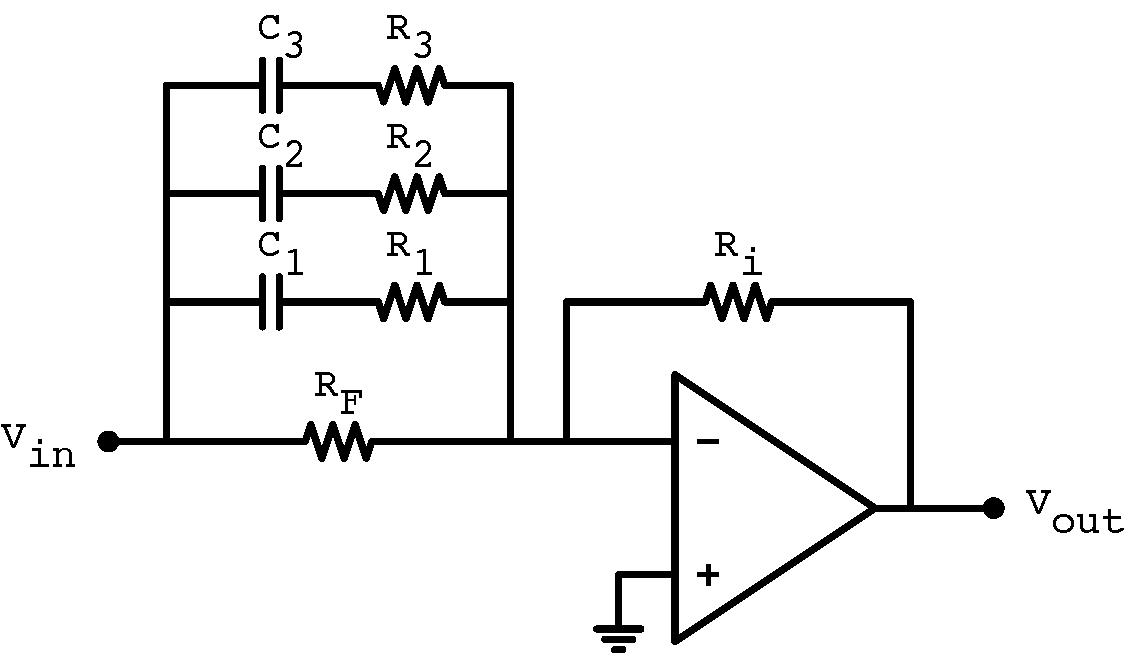
\includegraphics[resolution=300,scale=\circuitSize]{Figure/DesignAfFilter/FilterWithLess3.pdf}
	\caption{Kredsløbsdiagram for de tre filtre der skal dæmpe de lave frekvenser.}
	\label{fig:FilterDerDaemper}
\end{figure}
\noindent
%
Det eneste der ændre sig i forhold til forstærkningen af de lave frekvenser, er fortegnet på forstærkningen i dB, så istedet for at forstærke de lave frekvenser med 2.62dB skal der i disse filtre forstærkes med -2.62dB. Da det er den eneste forskel resulterer det ligeledes i at alle modstands- og kondensatorværdier er ens for de tre RC-led og afhænger kun af om forstærkningen er -2.62dB, -5.24dB eller -10.48dB.
%
\newpage
\noindent
%